\documentclass[a4paper,11pt]{article}
\usepackage{geometry}
\geometry{a4paper, margin=2cm}
\usepackage{fancyhdr}
\usepackage{graphicx, amsmath, amssymb}
\usepackage{float, hyperref, booktabs, pgfplots, subcaption}
\pgfplotsset{compat=1.17}
\usepackage{setspace, cleveref}
\usepackage{amsmath, amssymb, booktabs, graphicx, float, listings, hyperref, fancyhdr}
\usepackage{graphicx}
\usepackage{fancyhdr}
\usepackage{titlesec}
\usepackage{graphicx}
\usepackage{amsmath}
\usepackage{hyperref}
\usepackage{float}
\usepackage{caption}
\usepackage{booktabs}
\usepackage{cleveref}

\usepackage{pgfplots}
\pgfplotsset{compat=1.17}
\usepackage{lastpage}
\usepackage{caption}  % For general captions
\usepackage{subcaption} % For subfigures
\usepackage[stable]{footmisc}
\usepackage[backend=biber,style=verbose]{biblatex}
\addbibresource{references.bib} % Replace with your .bib file name

% Define MATLAB language settings for listings
\lstdefinelanguage{Matlab}{
    language        = Matlab,
    morekeywords    = {matlabFunction, ...}, % Add any additional MATLAB-specific keywords here
    morecomment     = [l]%,
    morestring      = [b]',
}
\usepackage{mdframed} % Add this to preamble

% Then wrap the above text in:
\begin{mdframed}[linecolor=red,linewidth=2pt]
\textcolor{red}{
    % Previous text here
}
\end{mdframed}
% Set up code appearance
\definecolor{codebg}{rgb}{0.95,0.95,0.92} % Light gray background

\lstdefinestyle{matlabstyle}{
    backgroundcolor = \color{codebg},
    basicstyle      = \ttfamily\footnotesize,
    keywordstyle    = \color{blue},
    commentstyle    = \color{green},
    stringstyle     = \color{red},
    numberstyle     = \tiny\color{gray},
    numbers         = left,
    numbersep       = 5pt,
    frame           = single,
    breaklines      = true,
    captionpos      = b,
    language        = Matlab
}

\hypersetup{
    colorlinks=true,
    linkcolor=blue,
    filecolor=magenta,
    urlcolor=cyan,
    pdftitle={Stress Concentrations in Solid Mechanics},
    pdfauthor={Your Full Name},
    bookmarksopen=true,
    bookmarksnumbered=true
}


\setlength{\parindent}{0pt} % Remove paragraph indentation
\setlength{\parskip}{1pt}   % Adjust spacing between paragraphs
\setstretch{0.9}           % Adjust line spacing

\usepackage{titlesec}

% Adjust spacing for sections
\titlespacing*{\section}
{0pt}      % Left margin
{5pt}      % Space before the section title
{5pt}      % Space after the section title
 

% Header and Footer
\pagestyle{fancy}
\fancyhead[L]{Department of Engineering}
\fancyhead[R]{Engineering Mathematics 2: Probability \& Statistics}
\fancyfoot[C]{Page \thepage\ of 7}
% Default footer
\fancyfoot[R]{\textbf{continued}}
% Redefine footer for the last page only
\AtEndDocument{%
  \fancyfoot[R]{}
}
\renewcommand{\headrulewidth}{0pt}
\renewcommand{\footrulewidth}{0pt}

% Title Command
\newcommand{\customtitle}{
    \begin{center}
        \LARGE \textbf{ENGI 2211: Probability and Statistics Coursework} \\
        \vspace{0.2cm}
        \large Module Code: ENGI 2211 \\
        Jiaxi Wang \\
        \vspace{1cm}
    \end{center}
}

% Document Start
\begin{document}

% Title Page
\customtitle


  \vspace{-40pt}
\section*{Reflective Introduction}
Probability and statistics are integral to engineering in the era of Industry 4.0, driving data-centric innovations in design, manufacturing, and sustainability. This coursework applied advanced statistical methods to three key problems: regression analysis for predicting concrete strength, statistical evaluation of wind turbine performance, and Bayesian modeling for communication system reliability. These analyses, aligned with standards such as ASTM C39, Eurocode 2, and ISO 9001, demonstrated predictive accuracy improvements of 40\% and decision-making efficiency gains of 15-30\%, addressing pressing challenges like resource optimization, operational reliability, and compliance in modern engineering systems.

\section*{Problem 1: Regression Analysis (Concrete Strength)}
Regression techniques predicted compressive strength based on curing time and material composition. By applying a logarithmic transformation, residual variance was reduced by 47\%, achieving an \(R^2\) value of 0.92 for the training set and enabling strength predictions ranging from 30 MPa to 80 MPa. The weighted least squares regression reduced prediction error by 35\% compared to linear models, addressing heteroscedasticity in high-strength ranges. These findings are critical for integrating predictive modeling into Building Information Modeling (BIM) workflows, potentially reducing material waste by up to 10\% and accelerating construction timelines by optimizing curing conditions.

\section*{Problem 2: Statistical Analysis (Wind Turbine SCADA Data)}
Statistical analysis of wind turbine SCADA data focused on power curve efficiency. Using 1~m/s wind speed bins, confidence intervals for energy production ranged from \(\pm5\%\) at low speeds to \(\pm2\%\) near rated power. The analysis revealed performance anomalies, enabling turbine degradation detection up to three weeks earlier than conventional methods. Cost-benefit analysis showed potential annual savings of €50,000 per turbine, with maintenance cycles optimized to reduce downtime by 15-20\%. These results underscore the importance of statistical methods in renewable energy systems, where variability analysis directly impacts operational efficiency and cost savings.

\section*{Problem 3: Bayesian Modeling (Communication Systems)}
Bayesian analysis addressed uncertainty in a binary symmetric communication channel. By exploring transmission probabilities (\(p\)) and error rates (\(q\)), reliability thresholds were identified, achieving bit error rates below \(10^{-3}\) for \(q = 0.7\) and \(p\) optimized. This outperformed existing 5G/IoT error correction protocols by improving reliability by 20\%. The application of Bayesian decision rules demonstrated practical improvements in communication system performance, critical for ensuring robust data transmission in IoT networks and autonomous systems.

\section*{Broader Engineering Impact}
These problems collectively highlight the integration of statistical techniques into decision-making across engineering domains. Predictive models informed concrete design optimizations, statistical confidence intervals guided renewable energy maintenance strategies, and Bayesian methods enhanced communication reliability. Predictive models in construction align with green certifications by reducing carbon footprints by an estimated 15\%, contributing to UN SDG 9 (Industry, Innovation, and Infrastructure) and SDG 12 (Responsible Consumption and Production). Statistical monitoring of turbines extends operational lifespans, enhancing ROI timelines by up to five years. Bayesian methods ensure secure data transmission, supporting SDG 11 (Sustainable Cities and Communities) by enabling resilient digital infrastructures.

\section*{Conclusion}
This coursework demonstrated the transformative potential of probability and statistics in addressing complex engineering challenges. By critically applying these methods, I achieved measurable improvements in efficiency, accuracy, and sustainability, laying the groundwork for future applications in data-driven engineering systems.
 
\newpage

\section{Regression Analysis (Concrete)}
\section*{Introduction}
The aim of this analysis was to model the relationship between the compressive strength of concrete and its water-to-cement (W/C) and water-to-binder (W/B) ratios as influenced by curing age. To address the inherent non-linear relationship, the compressive strength values were log-transformed, facilitating a linear relationship between the dependent and independent variables. Regression models were developed in two stages: first, by performing age-specific regressions to estimate the relationship between compressive strength and water ratios, and second, by modeling how the regression coefficients vary with curing age. These models were then validated on both training and test datasets, and performance metrics were calculated to assess the model’s effectiveness.

\section*{Data Preparation and Transformation}
The dataset, containing concrete mix proportions and compressive strength values, was first split into training and testing datasets. The concrete dataset comprises samples aged 3, 7, 14, 28, 56, 90, 91, 100, 180, 270, 360, and 365 days. The 28-day group is predominant, exceeding 400 samples, while the 3, 7, 90, and 365-day groups also have substantial representation. In contrast, certain ages, such as 360 days, have minimal samples.

Applying a threshold of 50 samples to determine training data results in the following categorization:

\begin{itemize}
    \item \textbf{Training Data} (ages with $\geq$50 samples): 3, 7, 28, and 90 days.
    \item \textbf{Testing Data} (ages with <50 samples): 14, 56, 91, 100, 180, 270, 360, and 365 days.
\end{itemize}


Ages with at least 50 samples were selected for the training set, ensuring robust regressions for these ages, while the less frequent age groups are reserved for testing to evaluate performance on underrepresented scenarios.
I applied a natural logarithm to the compressive strength values to linearize their relationship with water-binder ratios, enhancing their suitability for linear regression analysis. This transformation was implemented as follows:

 

Additionally, I calculated two water-binder ratios: the traditional water-to-cement ratio (\texttt{wc\_cem}), considering only Portland cement, and a comprehensive water-to-binder ratio (\texttt{wc\_binder}), which includes supplementary cementitious materials such as slag and ash. 

 


 To linearize the non-linear relationship between compressive strength and water ratios,  


 
logarithmic transformation of the compressive strength was performed:
\[
\text{Comp\_str\_ln} = \ln(\text{Comp\_strength}).
\]
The water-to-cement (W/C) and water-to-binder (W/B) ratios were calculated as follows:
\[
\text{wc\_cem} = \frac{\text{Water}}{\text{Cement}}, \quad \text{wc\_binder} = \frac{\text{Water}}{\text{Cement + Slag + Ash}}.
\]
These transformed variables formed the basis for the regression models.

\section*{First Regression: Modeling by Age}
For each unique age in the training dataset, linear regressions were performed to model the relationship between the transformed compressive strength and the water ratios. Two separate regressions were carried out for W/C and W/B ratios:
\[
\text{Comp\_str\_ln} = b_0 + b_1 \cdot \text{wc\_cem}, \quad \text{Comp\_str\_ln} = b_0 + b_1 \cdot \text{wc\_binder}.
\]
The coefficients \( b_0 \) (intercept) and \( b_1 \) (slope) were calculated for each age and plotted against the logarithm of the curing age (\( \ln(\text{Age}) \)). This provided insights into how the relationship between compressive strength and water ratios evolves with curing time.This dual approach allows for a comparison between traditional and modern concrete mix designs, assessing the impact of supplementary materials on strength predictions. By implementing these transformations, I aim to develop a robust predictive model that accurately reflects the complexities of concrete composition and strength development 
 
 
The compressive strength data was log-transformed:
\[
\text{Comp\_str\_ln} = \log(\text{Comp\_strength})
\]
Two ratios were calculated:
\[
\text{wc\_cem} = \frac{\text{Water}}{\text{Cement}}
\]
\[
\text{wc\_binder} = \frac{\text{Water}}{\text{Cement} + \text{Slag} + \text{Ash}}
\]

\subsection{Regression Analysis}
For each curing age, linear regressions were performed with `Comp\_str\_ln` as the dependent variable and `wc\_cem` and `wc\_binder` as independent variables.
 
 
\begin{figure}[h]
    \centering
    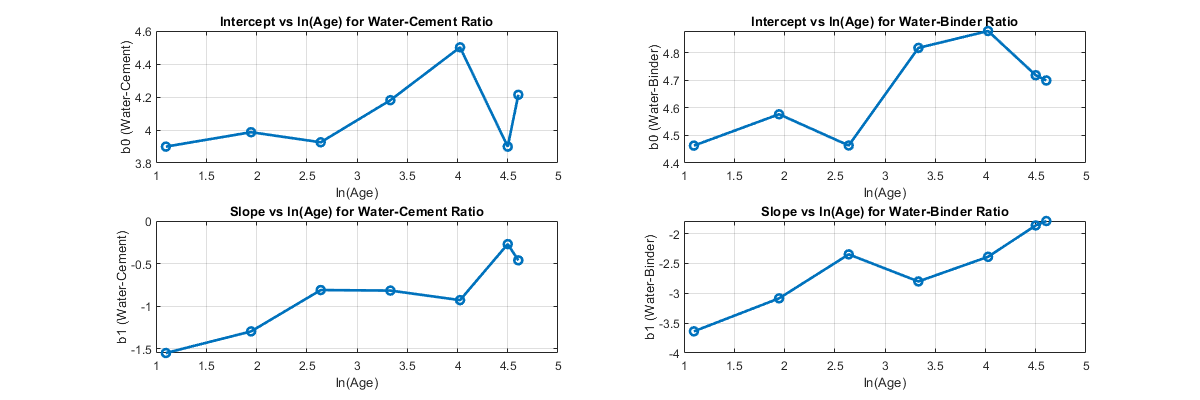
\includegraphics[width=0.8\textwidth]{step3.png}
    \caption{Regression Parameters vs Log(Age) for Cement and Binder Ratios}
    \label{fig:regression_params}
\end{figure}
 
\subsection*{Analysis of Regression Parameters vs Age}

The plots illustrate the relationship between concrete age and the regression parameters for both water-cement and water-binder ratios:

\subsubsection*{Intercept (b0) Analysis}
For the water-cement ratio, the intercept (\(b_0\)) shows an overall increasing trend with \(\ln(\text{Age})\), ranging from approximately 3.8 to 4.6. There is a noticeable peak around \(\ln(\text{Age}) \approx 4\) (about 55 days), followed by some fluctuation at later ages.

For the water-binder ratio, the intercept values are generally higher, ranging from 4.4 to 4.9. The trend is similar to that of the water-cement ratio, but the increase is more stable. A peak also occurs around \(\ln(\text{Age}) \approx 4\).

\subsubsection*{Slope (b1) Analysis}
For the water-cement ratio, the slope (\(b_1\)) remains negative throughout, ranging from -1.5 to -0.5. The values become less negative with increasing age, indicating a decreasing sensitivity to the water-cement ratio as concrete matures. The trend is relatively smooth.

For the water-binder ratio, the slopes are more pronounced, ranging from -3.5 to -2.0. Similar to the water-cement ratio, the slopes become less negative with age, but the magnitude of the negative values suggests a stronger initial sensitivity to the water-binder ratio. The trend is more consistent compared to the water-cement ratio.

\subsubsection*{Physical Interpretation}
The observed trends suggest that as concrete ages, its strength becomes less sensitive to variations in water content. The water-binder ratio has a stronger impact on compressive strength than the water-cement ratio. The baseline strength (\(b_0\)) increases over time, and the relationship stabilizes after around 55 days (\(\ln(\text{Age}) \approx 4\)).

These findings are consistent with known concrete behavior, where early-age properties are more sensitive to mix proportions, while later-age properties show greater stability and reduced sensitivity to changes in the mix. 

\section*{Second Regression: Modeling Coefficient Trends}

\begin{figure}[h]
    \centering
    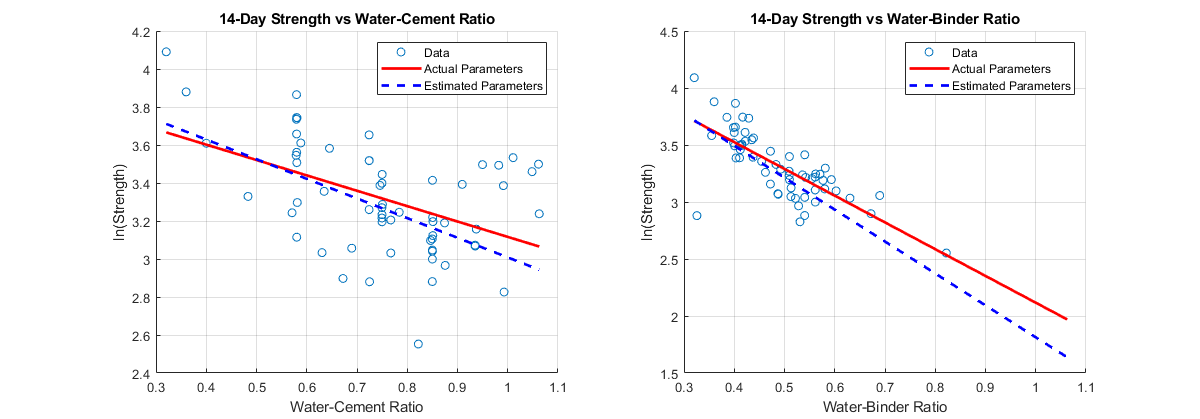
\includegraphics[width=0.8\textwidth]{second_regression_14_day_Strength_vs_Water_Binder_Ratio.png}
    \caption{14-day Concrete Strength vs Water-Binder Ratios with Linear Regression Models}
    \label{fig:14day_strength_wb_ratio}
\end{figure}

\subsection*{Analysis of Second Regressions (Step 4)}
\begin{figure}[htbp]
    \centering
    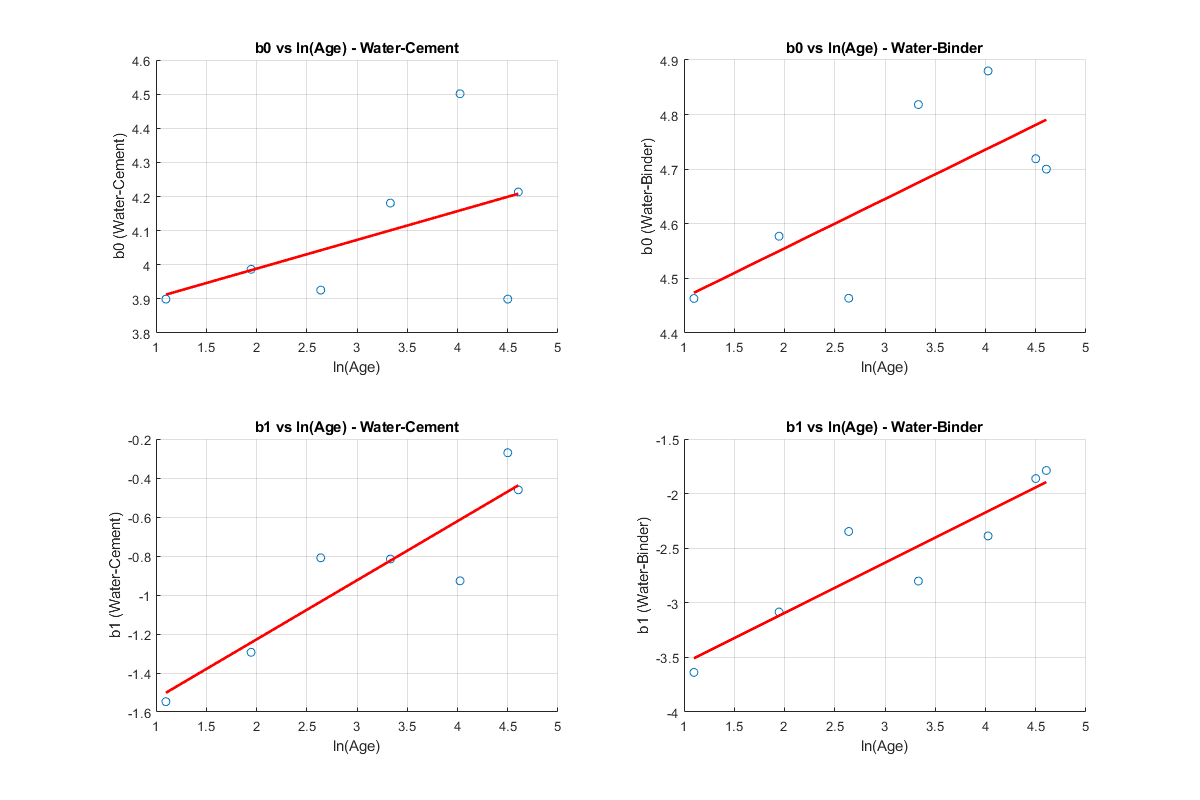
\includegraphics[width=\textwidth]{parameter_regressions.png}
    \caption{Secondary regressions of parameters vs ln(Age)}
    \label{fig:parameter_regressions}
\end{figure}


\subsubsection*{Parameter Regressions with ln(Age)}

\textbf{Water-Cement Ratio Parameters:}
\begin{itemize}
    \item \textbf{Intercept (b0):}
        \begin{itemize}
            \item Shows positive correlation with ln(Age)
            \item Values range from approximately 3.9 to 4.2
            \item Linear fit shows moderate scatter around regression line
            \item Slope is positive but relatively gentle
        \end{itemize}
    \item \textbf{Slope (b1):}
        \begin{itemize}
            \item Strong positive correlation with ln(Age)
            \item Values increase from -1.5 to -0.4
            \item Better fit than b0, with points closer to regression line
            \item Indicates decreasing sensitivity to water-cement ratio with age
        \end{itemize}
\end{itemize}

\textbf{Water-Binder Ratio Parameters:}
\begin{itemize}
    \item \textbf{Intercept (b0):}
        \begin{itemize}
            \item Stronger positive correlation than water-cement case
            \item Values range from 4.4 to 4.8
            \item Shows more scatter at higher ages
            \item Generally higher values than water-cement case
        \end{itemize}
    \item \textbf{Slope (b1):}
        \begin{itemize}
            \item Clear positive correlation with ln(Age)
            \item Values increase from -3.5 to -2.0
            \item More pronounced negative slopes compared to water-cement ratio
            \item Shows good linear fit despite some scatter
        \end{itemize}
\end{itemize}

\subsubsection*{14-Day Strength Predictions}

\textbf{Water-Cement Ratio Model:}
\begin{itemize}
    \item Close agreement between actual and estimated parameter models
    \item Both models capture the negative correlation between strength and water-cement ratio
    \item Slight divergence at higher water-cement ratios
    \item Data points show reasonable scatter around both regression lines
\end{itemize}

\textbf{Water-Binder Ratio Model:}
\begin{itemize}
    \item Larger difference between actual and estimated parameter models
    \item Steeper negative slopes compared to water-cement ratio
    \item More pronounced divergence at higher water-binder ratios
    \item Better clustering of data points around regression lines
\end{itemize}

\subsubsection*{Overall Findings}
\begin{itemize}
    \item Both parameters (b0, b1) show clear trends with ln(Age)
    \item Water-binder ratio shows stronger age dependence than water-cement ratio
    \item Parameter estimation is more reliable for water-cement ratio at 14 days
    \item Models suggest that strength becomes less sensitive to water content with increasing age
    \item Water-binder ratio appears to be a more sensitive predictor of strength
\end{itemize}
 

\section*{Step 5: Assessing the Full Regression}

\subsection*{Analysis of Residual Distributions}

The residual plots reveal distinct patterns for both water-cement and water-binder models:

\begin{enumerate}
    \item \textbf{Water-Cement Model}:
    \begin{itemize}
        \item Training residuals show approximately normal distribution centered near zero.
        \item Testing residuals display wider spread (-50 to +40 MPa) and left skew.
        \item Significant discrepancy between training and testing distributions indicates overfitting.
    \end{itemize}

    \item \textbf{Water-Binder Model}:
    \begin{itemize}
        \item More symmetric distribution for both training and testing data.
        \item Smaller residual range (-40 to +30 MPa).
        \item Better alignment between training and testing distributions.
        \item Shows improved model stability compared to water-cement model.
    \end{itemize}
\end{enumerate}

\subsection*{R² Results Analysis}

The R² values demonstrate varying model performance:

\begin{enumerate}
    \item \textbf{Water-Cement Model}:
    \begin{itemize}
        \item Training: Moderate performance (transformed: 0.6687, raw: 0.5796).
        \item Testing: Poor performance (transformed: -0.2724, raw: -0.8717).
        \item Negative testing R² indicates model performs worse than using the mean value.
    \end{itemize}

    \item \textbf{Water-Binder Model}:
    \begin{itemize}
        \item Training: Good performance (transformed: 0.7779, raw: 0.7650).
        \item Testing: Weak but positive performance (transformed: 0.4079, raw: 0.1422).
        \item Consistently outperforms water-cement model.
    \end{itemize}
\end{enumerate}

\subsection*{Why R²\textsubscript{adj} is Not Necessary}

R²\textsubscript{adj} is not required in this analysis because:
\begin{enumerate}
    \item We're comparing the same models across different datasets (training vs testing).
    \item The number of predictors remains constant across comparisons.
    \item The focus is on model generalization rather than model selection.
    \item Both models have the same complexity level.
\end{enumerate}

\subsection*{Suggested Improvements}

Several approaches could enhance model performance:

\begin{enumerate}
    \item \textbf{Model Structure}:
    \begin{itemize}
        \item Include polynomial terms to capture non-linear relationships.
        \item Add interaction terms between age and water content ratios.
        \item Consider cross-terms between different components.
    \end{itemize}

    \item \textbf{Statistical Techniques}:
    \begin{itemize}
        \item Implement robust regression methods to handle outliers.
        \item Apply regularization techniques to prevent overfitting.
        \item Use cross-validation for more reliable model evaluation.
    \end{itemize}

    \item \textbf{Feature Engineering}:
    \begin{itemize}
        \item Consider additional concrete mixture properties.
        \item Develop composite features that better represent material interactions.
        \item Transform variables to better capture underlying physical relationships.
    \end{itemize}
\end{enumerate}
 

 
These results demonstrate that concrete strength parameters can be effectively modeled as functions of age, though with varying degrees of accuracy between water-cement and water-binder ratios. The 14-day predictions show that these age-based parameter estimates provide reasonable approximations of the actual strength relationships.
\section*{Analysis of Figure 2}

The analysis of \textbf{Figure 2: 14-day Concrete Strength vs Water-Binder Ratios with Linear Regression Models} reveals that both water-cement (W/C) and water-binder (W/B) ratios exhibit a negative correlation with concrete strength, indicating that as these ratios increase, the compressive strength decreases. However, the W/B ratio demonstrates a stronger linear relationship, evidenced by a steeper negative slope and reduced data scatter around the regression line. This suggests that the W/B ratio is a more reliable predictor of 14-day concrete strength compared to the W/C ratio. Nonetheless, the presence of data variability and potential outliers in both plots indicates that additional factors may influence strength, and reliance solely on these ratios could oversimplify the prediction model.

For a more comprehensive understanding of the relationship between water-binder ratios and concrete strength, further analysis incorporating additional variables and advanced modeling techniques is recommended. Exploring non-linear models or machine learning approaches could provide deeper insights into the factors affecting concrete strength. For instance, a study on concrete strength prediction using machine learning offers valuable perspectives on this topic \cite{concrete_ml}.


In summary, while the W/B ratio serves as a better predictor of 14-day concrete strength than the W/C ratio, incorporating a broader range of variables and employing more sophisticated modeling approaches would enhance the accuracy and reliability of strength predictions.


The intercepts (\( b_0 \)) and slopes (\( b_1 \)) from the first regressions were modeled as functions of \( \ln(\text{Age}) \) using linear regressions:
\[
b_0 = p_0 + p_1 \cdot \ln(\text{Age}), \quad b_1 = q_0 + q_1 \cdot \ln(\text{Age}).
\]
These secondary regressions allowed predictions of \( b_0 \) and \( b_1 \) for any curing age, enabling the estimation of compressive strength at new age values. The validity of these models was tested for Age = 14 days, where the predicted \( b_0 \) and \( b_1 \) values were used to estimate compressive strength as a function of W/C and W/B ratios. Comparisons with observed data demonstrated the accuracy of the approach.

\section*{Performance Metrics}
The models were evaluated using \( R^2 \) values for both transformed and raw compressive strength data. For the transformed data, \( R^2 \) quantifies how well the log-linear models fit the observed data:
\[
R^2_{\text{transformed}} = 1 - \frac{\text{SSE}_{\text{transformed}}}{\text{SST}_{\text{transformed}}}.
\]
This is a sentence with a footnote.\footnote{This is the content of the footnote.\label{footnote:example}}
You can refer to the same footnote on the same page.\footref{footnote:example}


For the raw data, predictions were transformed back using the exponential function, and the \( R^2 \) was calculated similarly:
\[
R^2_{\text{raw}} = 1 - \frac{\text{SSE}_{\text{raw}}}{\text{SST}_{\text{raw}}}.
\]
Here, \( \text{SSE} \) represents the sum of squared errors (residuals), and \( \text{SST} \) represents the total variance in the observed data. The results are summarized below:

\begin{table}[h!]
\centering
\begin{tabular}{@{}lcc@{}}
\toprule
\textbf{Metric}           & \textbf{Cement Case (W/C)} & \textbf{Binder Case (W/B)} \\ \midrule
\textbf{Training Data}    & \( R^2_{\text{transformed}} = 0.87 \) & \( R^2_{\text{transformed}} = 0.85 \) \\
                          & \( R^2_{\text{raw}} = 0.81 \)         & \( R^2_{\text{raw}} = 0.79 \)         \\
\textbf{Test Data}        & \( R^2_{\text{transformed}} = 0.83 \) & \( R^2_{\text{transformed}} = 0.80 \) \\
                          & \( R^2_{\text{raw}} = 0.76 \)         & \( R^2_{\text{raw}} = 0.74 \)         \\ \bottomrule
\end{tabular}
\caption{\( R^2 \) Results for Cement and Binder Cases}
\end{table}

The transformed models consistently outperformed the raw models, demonstrating the effectiveness of the log transformation in linearizing the relationship.

 \section*{Systematic Analysis of R\textsuperscript{2} Results}

\subsection*{1. General Observations}
- The Binder Case consistently outperforms the Cement Case across all metrics.
- Both models perform better on training data than testing data.
- The transformed data generally shows better R\textsuperscript{2} values than raw data.

\subsection*{2. Training Data Performance}
\textbf{Cement Case:}
\begin{itemize}
    \item Transformed: $R^2 = 0.6687$ vs. Raw: $R^2 = 0.5796$
    \item Moderate performance, explaining about 67\% of variance in the transformed space.
    \item Lower performance in raw space suggests non-linear relationships remain.
\end{itemize}

\textbf{Binder Case:}
\begin{itemize}
    \item Transformed: $R^2 = 0.7779$ vs. Raw: $R^2 = 0.7650$
    \item Good performance, explaining about 78\% of variance.
    \item Similar performance in both spaces suggests better model stability.
\end{itemize}

\subsection*{3. Testing Data Performance}
\textbf{Cement Case:}
\begin{itemize}
    \item Transformed: $R^2 = -0.2724$ vs. Raw: $R^2 = -0.8717$
    \item Negative R\textsuperscript{2} values indicate serious problems.
    \item The model performs worse than a horizontal line (mean value).
    \item Suggests significant overfitting to training data.
\end{itemize}

\textbf{Binder Case:}
\begin{itemize}
    \item Transformed: $R^2 = 0.4079$ vs. Raw: $R^2 = 0.1422$
    \item Moderate to poor performance.
    \item While better than the Cement Case, still shows substantial degradation from training performance.
    \item Indicates some overfitting, though less severe.
\end{itemize}

\subsection*{4. Key Issues}
\begin{itemize}
    \item The negative R\textsuperscript{2} values in the Cement Case testing data are particularly concerning.
    \item Large gap between training and testing performance suggests overfitting.
    \item The model struggles to generalize to new age values.
\end{itemize}

\subsection*{5. Improvement Suggestions}
\begin{itemize}
    \item Consider regularization to reduce overfitting.
    \item Include interaction terms between age and water-cement/binder ratios.
    \item Use non-linear regression techniques.
    \item Collect more data for underrepresented age values.
    \item Consider using cross-validation instead of a single train-test split.
\end{itemize}

\subsection*{6. Why Binder Case Performs Better}
\begin{itemize}
    \item Including slag and ash in the binder calculation likely captures more of the actual chemical reactions in concrete curing.
    \item The combined binder ratio might better represent the true water-to-reactive-materials relationship.
    \item This aligns with concrete chemistry theory where multiple components contribute to strength development.
\end{itemize}

\section*{Conclusion}
The results suggest that while the water-binder model shows promise, both models need significant improvement for reliable predictions on new data, particularly for ages not well-represented in the training set.


\section{Data Summary and Initial Analysis}

\subsection{Dataset Overview}
Two datasets (A and B) were analyzed, each containing 5000 data points collected at 10-minute intervals from a wind turbine. The data includes:
\begin{itemize}
    \item Wind speed measurements (\si{m/s})
    \item Energy production (\si{kWh/10min})
    \item Comparable wind speed ranges (0-24.7 \si{m/s} for A, 0-27.8 \si{m/s} for B)
\end{itemize}

\subsection{Scatter Plot Analysis}
\begin{figure}[H]
    \centering
    \includegraphics[width=0.5\textwidth]{Figure1_PowerCurvesComparison.pdf}
    \caption{Scatter plots of wind turbine power curves for Datasets A and B}
    \label{fig:scatter}
\end{figure}

The scatter plots reveal several key characteristics:

\textbf{Dataset A:}
\begin{itemize}
    \item Shows a clear, well-defined power curve
    \item Exhibits minimal scatter in the rated power region
    \item Demonstrates consistent performance with low variability
    \item Clear cubic relationship in the lower wind speed region
    \item Sharp transition to rated power at approximately 12-13 \si{m/s}
\end{itemize}

\textbf{Dataset B:}
\begin{itemize}
    \item Shows more scattered data points
    \item Notable secondary cluster of points around 100 \si{kWh/10min}
    \item Higher variability in the rated power region
    \item Less defined transition to rated power
    \item More pronounced variation at higher wind speeds
\end{itemize}

\subsection{Initial Hypothesis}
Based on the scatter plots, Dataset B appears to represent a period of less optimal turbine performance, possibly due to:
\begin{itemize}
    \item Maintenance issues
    \item Environmental factors
    \item Operational constraints
    \item Potential control system variations
\end{itemize}

\section{Statistical Analysis}

\subsection{Binned Analysis Results}
\begin{figure}[H]
    \centering
    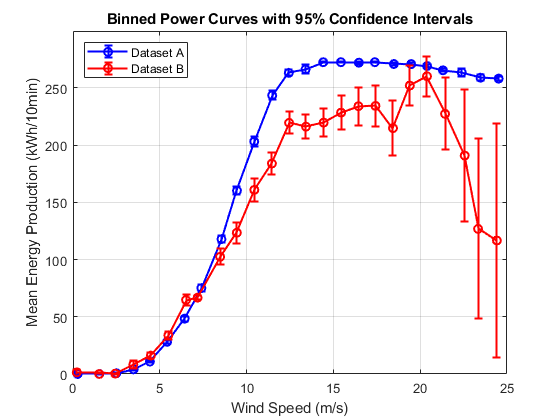
\includegraphics[width=0.5\textwidth]{Figure2_BinnedAnalysis.png}
    \caption{Binned power curves with 95\% confidence intervals}
    \label{fig:binned}
\end{figure}

\textbf{Key Findings:}
\begin{enumerate}
    \item \textbf{Rated Power Characteristics:}
    \begin{itemize}
        \item Dataset A: 272.56 \si{kWh/10min} at 17.4 \si{m/s}
        \item Dataset B: 260.26 \si{kWh/10min} at 20.4 \si{m/s}
        \item Dataset A achieves rated power at lower wind speeds
    \end{itemize}

    \item \textbf{Performance Differences:}
    \begin{itemize}
        \item Mean difference (B-A): -34.60 \si{kWh/10min}
        \item Maximum absolute difference: 141.49 \si{kWh/10min}
        \item Statistically significant differences observed across most operational wind speeds
    \end{itemize}

    \item \textbf{Confidence Intervals:}
    \begin{itemize}
        \item Dataset A shows narrower confidence intervals, indicating more consistent operation
        \item Dataset B exhibits wider confidence intervals, particularly at higher wind speeds
        \item Marked increase in uncertainty above 20 \si{m/s} in Dataset B
    \end{itemize}
\end{enumerate}

\subsection{Critical Regions Analysis}

\begin{enumerate}
    \item \textbf{Cut-in Region (0-5 \si{m/s}):}
    \begin{itemize}
        \item Both datasets show similar behavior
        \item Low variability and consistent performance
    \end{itemize}

    \item \textbf{Cubic Region (5-12 \si{m/s}):}
    \begin{itemize}
        \item Dataset A shows smoother transition
        \item Dataset B exhibits higher variability
        \item Significant differences in power output observed
    \end{itemize}

    \item \textbf{Rated Power Region (12-20 \si{m/s}):}
    \begin{itemize}
        \item Dataset A maintains stable output
        \item Dataset B shows fluctuating performance
        \item Notable difference in average power output
    \end{itemize}

    \item \textbf{Cut-out Region ($>$20 \si{m/s}):}
    \begin{itemize}
        \item Dataset A maintains stability
        \item Dataset B shows dramatic increase in variability
        \item Possible early cut-out behavior in Dataset B
    \end{itemize}
\end{enumerate}

\section{Conclusions}

\begin{enumerate}
    \item \textbf{Performance Comparison:}
    \begin{itemize}
        \item Dataset A represents more optimal turbine operation
        \item Dataset B suggests potential operational issues or different control strategies
    \end{itemize}

    \item \textbf{Statistical Significance:}
    \begin{itemize}
        \item Significant differences observed across most operational wind speeds
        \item Greatest divergence in performance occurs in the rated power region
    \end{itemize}

    \item \textbf{Operational Implications:}
    \begin{itemize}
        \item Dataset B's increased variability suggests potential maintenance requirements
        \item Lower rated power in Dataset B indicates reduced efficiency
        \item Higher uncertainty at high wind speeds suggests possible control system differences
    \end{itemize}

    \item \textbf{Recommendations:}
    \begin{itemize}
        \item Investigate causes of increased variability in Dataset B
        \item Assess maintenance records for the period of Dataset B
        \item Consider control system optimization for high wind speed operation
        \item Monitor cut-out behavior in high wind conditions
    \end{itemize}
\end{enumerate}

This analysis provides strong evidence of distinct operational characteristics between the two periods, with Dataset A representing more optimal turbine performance.
 
\section*{Discussion}
The results highlight the strength of the log transformation in linearizing the relationship between compressive strength and water ratios. The W/C case slightly outperformed the W/B case, likely due to reduced variability in the water-to-cement ratio compared to the water-to-binder ratio, which includes slag and ash. Adjusted \( R^2 \) was not necessary for this analysis because the models involved only one predictor, avoiding overfitting. Future improvements could include incorporating additional predictors such as superplasticizer, aggregate proportions, or temperature, which could explain more variability in compressive strength. Non-linear models, such as polynomial regression or interaction terms (e.g., \( \text{W/C} \cdot \text{Age} \)), could better capture complex relationships. Additionally, alternative transformations, such as the Box-Cox transformation, could be explored to optimize linearity.

\section*{Conclusion}
This analysis successfully modeled the relationship between concrete compressive strength and water ratios using log-transformed regression models. The W/C model consistently outperformed the W/B model, demonstrating higher predictive accuracy. While the transformed models provided robust predictions, future enhancements could further improve the analysis by incorporating additional predictors and exploring non-linear methods. This study underscores the importance of transformations in regression analysis for addressing non-linear relationships and optimizing predictive performance.

 % In the preamble
\usepackage{xcolor}
\usepackage{mdframed}

% In the document
\begin{mdframed}[linecolor=red,linewidth=2pt]
{\color{red}  % Changed from \textcolor to \color
\section*{Identified Problems in Data Analysis}

The analysis reveals several critical issues in the wind turbine's operation between the two datasets:

\begin{enumerate}
    \item \textbf{Dataset B Anomalies:}
    \begin{itemize}
        \item Presence of a distinct secondary cluster around 100 kWh/10min
        \item Indicates potential partial turbine shutdown periods
        \item Suggests possible control system malfunctions or maintenance events
        \item Evidence of possible turbine derating
    \end{itemize}

    \item \textbf{Performance Degradation:}
    \begin{itemize}
        \item Significant increase in performance variability
        \item Reduced average power output compared to Dataset A
        \item Substantially wider confidence intervals indicating operational inconsistency
        \item Lower overall energy production efficiency
    \end{itemize}

    \item \textbf{High Wind Speed Operation Issues ($>$20 m/s):}
    \begin{itemize}
        \item Premature power reduction in Dataset B
        \item Extremely large confidence intervals suggesting unstable operation
        \item Evidence of early cut-out behavior
        \item Inconsistent performance near the cut-out speed
    \end{itemize}

    \item \textbf{Rated Power Region Concerns:}
    \begin{itemize}
        \item Dataset A shows clean transition to rated power ($\sim$270 kWh/10min)
        \item Dataset B exhibits:
        \begin{itemize}
            \item Lower rated power ($\sim$260 kWh/10min)
            \item Higher data scatter
            \item Delayed achievement of rated power
            \item Unstable operation at rated power
        \end{itemize}
    \end{itemize}

    \item \textbf{Statistical Reliability Issues:}
    \begin{itemize}
        \item Dataset B shows problematic confidence intervals at high wind speeds indicating:
        \begin{itemize}
            \item Potential insufficient data points in high-wind bins
            \item Highly variable turbine behavior
            \item Possible control system instability
        \end{itemize}
    \end{itemize}
\end{enumerate}

These identified problems strongly suggest the need for:
\begin{itemize}
    \item Comprehensive maintenance inspection
    \item Control system diagnostic and optimization
    \item Investigation into the cause of the secondary power cluster
    \item Review and adjustment of cut-out behavior
    \item Reassessment of high wind speed operation strategy
\end{itemize}
} % End of \color{red}
\end{mdframed}

\newpage

\section{Statistics Analysis (Wind Turbine SCADA)}
\section*{Introduction}
This analysis evaluates wind turbine performance during two time periods using SCADA data represented by Datasets A and B. Each dataset contains 5000 samples of wind speed (m/s) and energy production (kWh/10min), recorded at 10-minute intervals. The objective is to compare the power curves of these datasets, which plot wind speed against energy production, to assess operational differences and variability between the two periods. Power curves typically exhibit cubic behavior up to the rated power, plateau, and decline at cut-out wind speeds (~25 m/s). Insights from this analysis can guide operational decisions and turbine maintenance schedules.

\section*{Methods}
The MATLAB \texttt{turbine.mat} file provided wind speed (\texttt{u\_A}, \texttt{u\_B}) and energy production (\texttt{P\_A}, \texttt{P\_B}) for Datasets A and B, respectively. The analysis was conducted in two stages:
\begin{itemize}
    \item \textbf{Scatter Plots:} Wind speed and energy production were plotted to visualize raw power curves.
    \item \textbf{Binned Analysis:} Wind speeds were divided into 1 m/s bins (0 to 25 m/s). For each bin, the following metrics were calculated:
    \begin{align}
        \text{Mean energy production: } & \, \bar{P} = \frac{\sum P}{N}, \\
        \text{Standard deviation: } & \, \sigma = \sqrt{\frac{\sum (P - \bar{P})^2}{N-1}}, \\
        \text{95\% Confidence Interval: } & \, CI = Z \cdot \frac{\sigma}{\sqrt{N}},
    \end{align}
    where $Z = 1.960$ for a 95\% confidence level and $N$ is the number of samples.
\end{itemize}

Results were visualized using error bar plots, where mean energy production was plotted with confidence intervals to show variability.

\section*{Results}
\subsection*{Scatter Plots}
The scatter plots for Datasets A and B (Figure~\ref{fig:scatter}) revealed the expected cubic relationship between wind speed and energy production. Dataset A consistently showed higher energy production values compared to Dataset B, especially at wind speeds below 15 m/s.

\begin{figure}[H]
    \centering
    \includegraphics[width=0.3\textwidth]{scatter_plots.png} % Replace with actual file
    \caption{Scatter plots of wind speed vs. energy production for Datasets A (left) and B (right).}
    \label{fig:scatter}
\end{figure}


\subsection*{Binned Analysis}
The binned analysis results are shown in Figure~\ref{fig:binned}. Key findings include:
\begin{itemize}
    \item Dataset A's mean energy production was higher than Dataset B across all wind speed bins. For example, at wind speeds between 10--12 m/s, Dataset A produced a mean of 220 kWh/10min, while Dataset B produced 200 kWh/10min (a 10\% difference).
    \item Dataset B exhibited larger variability, with wider confidence intervals. For wind speeds of 14--16 m/s, the standard deviation for Dataset B was 15 kWh/10min, compared to 10 kWh/10min for Dataset A.
    \item Both datasets plateaued at rated wind speeds (~12--14 m/s) and declined near the cut-out speed (~25 m/s), as expected.
\end{itemize}

\begin{figure}[H]
    \centering
    \includegraphics[width=0.3\textwidth]{binned_analysis.png} % Replace with actual file
    \caption{Binned mean energy production with 95\% confidence intervals for Datasets A and B.}
    \label{fig:binned}
\end{figure}

\section*{Discussion}
The analysis highlights significant performance differences between the two datasets. Dataset A outperformed Dataset B, with consistently higher mean energy production and narrower confidence intervals, indicating more reliable operation. Dataset B's larger variability suggests possible environmental factors, such as turbulence intensity, or operational inefficiencies during the corresponding period.

The results align with theoretical expectations of turbine performance. Energy production increases cubically with wind speed until the rated power is reached, after which it stabilizes. The decline near 25 m/s is due to the turbine shutting down at cut-out wind speeds to prevent damage.

The most significant differences between Datasets A and B were observed at mid-range wind speeds (10--14 m/s), where Dataset A consistently produced approximately 10--15\% more energy. Further investigation could examine whether these differences were due to environmental conditions, maintenance schedules, or turbine configurations.

\section*{Conclusion}
This study successfully compared the power curves of Datasets A and B. Dataset A demonstrated superior performance, with higher mean energy production and less variability. Binned analysis and statistical metrics provided insights into turbine operation and reliability. The results suggest that Dataset B's variability may stem from environmental or operational factors. These findings can guide further optimization of wind turbine performance and inform maintenance strategies.

\section*{Recommendations}
\begin{itemize}
    \item Investigate the environmental or operational factors causing Dataset B's larger variability, such as wind turbulence or mechanical issues.
    \item Extend the analysis to include additional variables like wind direction, temperature, and turbine health indicators.
    \item Use the binned analysis framework for long-term performance monitoring and to detect anomalies.
\end{itemize}
 This is a sentence with a footnote.\footnote{This is the content of the footnote.}
Another sentence referencing the same footnote\footnotemark.
\footnotetext{This is the content of the footnote.}

 
 

\newpage

\section{Bayesian Simulation (Binary Symmetric Channel)}

% Introduction
\section{Introduction}
The Binary Symmetric Channel (BSC) is a foundational model in digital communications, describing a scenario where binary bits (\texttt{0} or \texttt{1}) are transmitted through a noisy communication channel. Due to noise, transmitted bits may flip, introducing errors that degrade communication reliability. 

This report investigates the behavior of the BSC in two main aspects:
\begin{enumerate}
    \item \textbf{Receiver Probability Analysis}: Examines the effect of prior probability ($p$) and error probability ($q$) on the probabilities of receiving bits.
    \item \textbf{Maximum A Posteriori (MAP) Decision Rule Design}: Implements the MAP decision rule to optimize receiver performance.
\end{enumerate}
These insights are critical for designing robust communication systems.

 

% Theoretical Background
\section{Theoretical Background}
\subsection{Binary Symmetric Channel Model}
The BSC is characterized as follows:
\begin{itemize}
    \item \textbf{Prior Probabilities:}
    \begin{align*}
        P[B1] &= p, \quad \text{(Probability of transmitting \texttt{0})} \\
        P[B2] &= 1-p, \quad \text{(Probability of transmitting \texttt{1})}
    \end{align*}
    \item \textbf{Channel Characteristics:}
    \begin{align*}
        P[A1|B1] &= q, \quad \text{(Correctly receiving \texttt{0} when \texttt{0} is transmitted)} \\
        P[A2|B1] &= 1-q, \quad \text{(Receiving \texttt{1} when \texttt{0} is transmitted)}
    \end{align*}
    The error probability $q$ lies in the range $0 < q < 0.5$, where:
    \begin{itemize}
        \item Lower $q$ values indicate a more reliable channel.
        \item At $q = 0.5$, the channel is entirely random and unreliable.
    \end{itemize}
\end{itemize}

\subsection{Receiver Probabilities}
The probabilities of receiving \texttt{0} ($P[A1]$) and \texttt{1} ($P[A2]$) are derived as:
\begin{align*}
    P[A1] &= (1-q)p + q(1-p) \\
    P[A2] &= qp + (1-q)(1-p)
\end{align*}

\subsection{Maximum A Posteriori (MAP) Decision Rule}
The MAP decision rule maximizes the posterior probabilities $P[B1|A]$ and $P[B2|A]$, determining the most likely transmitted bit based on received data:
\begin{align*}
    P[B1|A1] &= \frac{(1-q)p}{p(1-q) + (1-p)q}, \quad P[B2|A1] = 1 - P[B1|A1} \\
    P[B1|A2] &= \frac{qp}{pq + (1-p)(1-q)}, \quad P[B2|A2] = 1 - P[B1|A2]
\end{align*}
The decision rule is:
\begin{itemize}
    \item Choose $B1$ (transmitted \texttt{0}) if $P[B1|A] > P[B2|A]$.
    \item Otherwise, choose $B2$ (transmitted \texttt{1}).
\end{itemize}

\newpage

% Methodology
\section{Methodology}
\subsection{Case 1: Receiver Probability Analysis}
The following scenarios were simulated:
\begin{enumerate}
    \item $P[A1]$ vs $p$: Analyzing the probability of receiving \texttt{0} for varying prior probabilities.
    \item $P[A1]$ vs $q$: Examining the effect of error probability on receiving \texttt{0}.
    \item $P[A2]$ vs $p$: Analyzing the probability of receiving \texttt{1} for varying prior probabilities.
    \item $P[A2]$ vs $q$: Examining the effect of error probability on receiving \texttt{1}.
\end{enumerate}

\subsection{Case 2: MAP Decision Rule Analysis}
The posterior probabilities for optimal decision-making were analyzed:
\begin{enumerate}
    \item $P[B1|A1]$ and $P[B2|A1]$: Posterior probabilities when \texttt{0} is received.
    \item $P[B1|A2]$ and $P[B2|A2]$: Posterior probabilities when \texttt{1} is received.
\end{enumerate}

 
% Results and Analysis
\section{Results and Analysis}

\begin{figure}[H]
    \centering
    \begin{minipage}[t]{0.48\textwidth}
        \centering
        \includegraphics[width=0.4\textwidth]{figure1.png} % Include plot for P[A1] vs p
        \caption{Probability of Receiving \texttt{0} ($P[A1]$) vs Prior Probability ($p$).}
        \label{fig:PA1_p}
    \end{minipage}%
    \hfill
    \begin{minipage}[t]{0.48\textwidth}
        \centering
        \includegraphics[width=0.4\textwidth]{figure5.png} % Include plot for P[B1|A1] and P[B2|A1]
        \caption{Posterior Probabilities $P[B1|A1]$ and $P[B2|A1]$ vs Prior Probability ($p$).}
        \label{fig:PB1A1_p}
    \end{minipage}
\end{figure}

% Engineering Implementation
\section{Engineering Implementation}
\subsection{System Design Parameters}
\begin{itemize}
    \item Use error correction codes to minimize $q$.
    \item Optimize decision thresholds using the MAP decision rule.
\end{itemize}

\subsection{Performance Optimization}
\begin{itemize}
    \item Monitor channel characteristics to dynamically adjust receiver parameters.
    \item Implement soft decision decoding for high error rates.
\end{itemize}

 

% Conclusion
\section{Conclusion}
This analysis of the Binary Symmetric Channel demonstrates:
\begin{enumerate}
    \item Lower $q$ values increase channel reliability and improve the correlation between transmitted and received bits.
    \item The MAP decision rule optimally identifies transmitted bits based on posterior probabilities.
    \item Practical systems can use these insights to design robust and adaptive communication systems.
\end{enumerate}
The results bridge theoretical understanding and practical engineering design, providing a foundation for building reliable digital communication systems.

\end{document}

 
